\documentclass[11pt,a4paper]{article}
\usepackage[margin=2.5cm]{geometry}
\usepackage[T1]{fontenc}
\usepackage[utf8]{inputenc}
\usepackage{booktabs,graphicx,amsmath,amssymb}
\usepackage[hidelinks]{hyperref}
\usepackage{natbib}
\usepackage{caption}
\captionsetup{font=small,labelfont=bf}
\usepackage{enumitem}
\setlength{\parskip}{2pt}

\title{\textbf{Performance--cost balance in large language model multi-agent
systems for medical examination question answering:\\ a systematic review}}
\author{[Author list to be completed]}
\date{Draft v0.1 --- \today}

\begin{document}
\maketitle

\begin{abstract}
\noindent\textbf{Background.} Large language model (LLM) multi-agent systems (MAS) are
increasingly proposed for medical question answering. Published frameworks are almost
uniformly optimised for accuracy, while the inference cost they incur is rarely measured and
almost never traded off explicitly.

\noindent\textbf{Objectives.} To determine (i) what single-agent baselines and evaluation
slices the literature actually uses, (ii) how accuracy gain and cost vary with the number of
agents and backbone model scale, (iii) which collaboration mechanisms buy accuracy cheaply,
and (iv) how gains vary with item difficulty.

\noindent\textbf{Methods.} We searched PubMed and arXiv (2022-01-01 to 2026-09-23),
supplemented by Google Scholar, ACL Anthology and forward citation chasing, for LLM-based
multi-agent systems evaluated on text-based medical examination question answering.
Peer-reviewed publications were prioritised and the publication status of every record was
verified against Semantic Scholar and OpenAlex. The primary outcome is a \emph{pair}: the
within-study paired accuracy difference $\Delta\mathrm{Acc}$ against a matched single-agent
baseline, and the cost ratio $R$. Because comparisons cluster within studies, the study --
not the comparison -- is the unit of inference; uncertainty is quantified by a
study-clustered bootstrap.

\noindent\textbf{Results.} 2{,}288 deduplicated records yielded 343 for manual review and
202 retrievable full texts. Thirty studies contributed 293 extractable comparisons, 280 of
them from peer-reviewed sources. Restricted to exam-style medical multiple-choice accuracy,
peer-reviewed sources and systems whose multi-agent contribution is separable from
fine-tuning, \textbf{93 comparisons from 13 studies} were available against the strongest
single-agent configuration reported in the same study. The comparison-level median was
$-1.73$ pp (IQR $-4.62$ to $+0.64$; 69\% negative; only 14\% exceeded the pre-specified
2 pp threshold), the \textbf{study-level median was $-0.31$ pp} (7 of 13 studies negative),
and the study-clustered bootstrap 95\% CI for the pooled median was
$\mathbf{[-2.70, +0.36]}$, \textbf{which includes zero}. The reported benefit fell
monotonically with comparator strength: $+8.4$ pp against chain-of-thought with
self-consistency, $+7.7$ against zero-shot, $+4.7$ against a same-scale single model,
$+1.9$ against the same backbone without retrieval, and $-1.7$ against the strongest single
agent. Typical cost was a median $R$ of $4\times$. Gains concentrated on hard items: against
a same-backbone single agent the median effect was $-3.1$ pp on Basic items, $-2.2$ on
Intermediate and $+1.4$ on Expert.

\noindent\textbf{Conclusions.} There is \emph{no reproducible accuracy advantage} for medical
multi-agent systems once the comparator is the strongest single agent the same paper already
ran; the direction is robust across every sensitivity analysis but the magnitude is not.
Reporting of cost is so incomplete that cost had to be derived from architecture in most
comparisons. We recommend that future work report a same-backbone strongest baseline, an
equal-budget self-consistency control arm, and per-question cost as a matter of course.

\noindent\textbf{Registration.} Protocol in \texttt{design/plan.md}; \emph{not}
prospectively registered (see \S\ref{sec:limproc}).
\end{abstract}

\section{Introduction}

Since instruction-tuned LLMs began to approach passing scores on medical licensing
examinations, a large family of \emph{multi-agent} systems has been proposed: panels of
specialist personas, debating agents, generator--critic pairs, hierarchical coordinators and
heterogeneous model ensembles. The rhetorical structure of these papers is remarkably
uniform: a new orchestration is introduced, evaluated on MedQA, MedMCQA or the medical
subsets of MMLU, and shown to exceed some single-model baseline.

Two things are almost always missing. First, the \textbf{cost} of the orchestration.
A system that issues seven model calls per question is not comparable with one that issues
a single call, yet accuracy is typically reported as if it were. Second, a \textbf{fair
comparator}. When the baseline is a zero-shot prompt while the proposed system uses
chain-of-thought reasoning, several rounds of sampling, retrieval and an aggregation step,
the reported ``multi-agent gain'' confounds collaboration with everything else that was
added.

This review therefore does not ask \emph{which framework is best}. It asks where the
\textbf{balance} lies: what combination of model scale, agent count, mechanism and item
difficulty buys a meaningful accuracy gain at an acceptable cost.

\paragraph{Research questions.}
\begin{description}[leftmargin=2.2em,itemsep=1pt]
\item[RQ1] Which baselines, dataset slices and sampling procedures does the literature use,
and how comparable are the resulting evaluation groups?
\item[RQ2] How do $\Delta\mathrm{Acc}$, $R$ and $\mathrm{CEI}$ vary with the number of agents
and backbone scale?
\item[RQ3] Which mechanisms (debate, role specialisation, retrieval, heterogeneity,
verification, aggregation) deliver accuracy cheaply?
\item[RQ4] How do gains vary with item difficulty?
\end{description}

\section{Methods}

\subsection{Protocol and reporting}
The review follows PRISMA 2020 for reporting, PRISMA-S for the search, and SWiM for
synthesis without meta-analysis. The protocol is version-controlled in
\texttt{design/plan.md}. Deviations from it are listed in \S\ref{sec:limproc}.

\subsection{Eligibility criteria}
\textbf{Included:} studies evaluating an LLM-driven system in which at least two agents
exchange information before producing an answer (or an internal ablation of such a system),
reporting accuracy on a text-based medical examination-style multiple-choice benchmark,
first released on or after 2022-01-01, in English or Chinese.
\textbf{Publication type:} peer-reviewed journal articles and papers accepted at
peer-reviewed conferences (in this field the conference \emph{is} the venue of record) were
prioritised. Preprints were retained in the register but enter the primary analysis only when
the evidence they contain is not available from a peer-reviewed source; every extracted row
carries its publication status.
\textbf{Excluded:} primarily multimodal inputs; primarily open-ended generation without an
objective key; no extractable numerical result; and systems for which the multi-agent
contribution cannot be separated from retrieval, tools or extra sampling \emph{and} which
report no ablation.

\subsection{Information sources and search}
The search was run in two layers. The \textbf{horizontal layer} covered all four research
questions plus the cross-cutting cost dimension; the \textbf{vertical layer} deepened each
dimension with question-specific terminology, giving a matrix of 35 queries
(RQ1 evaluation and baselines, 6; RQ2 agent count and model scale, 7; RQ3 mechanisms, 10;
RQ4 difficulty, 6; cost and efficiency, 6). The matrix was executed against three
bibliographic APIs and, in addition, against Google Scholar through a browser, because
Scholar indexes conference proceedings (ACL Anthology, AAAI, NeurIPS, ICASSP, ACM) that the
other sources cover unevenly.

Sources and yields: PubMed (E-utilities, 752 records), OpenAlex (matrix queries, 461+
records), arXiv (facet queries, supplementary probes and the full matrix, 2{,}592 records),
Google Scholar (69 harvested records with venue and citation counts), and forward citation
chasing through the Semantic Scholar graph on six seed papers (MedAgents, MDAgents,
MedAgentBoard, \emph{More agents is all you need}, multi-agent debate, Medprompt), which
returned 722 citing works. All searched to 2026-09-23.

Google Scholar proved decisive: it surfaced 34 records absent from the API corpus,
including the most-cited works in the field and an entire cost-aware multi-agent literature
(token-distribution benchmarking, budgeted routing, cost-aware agent pruning) that the
medical-facing queries had missed. Open-access full texts of peer-reviewed articles were obtained through
PubMed Central and through open-access links resolved via OpenAlex.
Publication status of every arXiv record was verified against the Semantic Scholar
batch API, which identified 28 of 101 retrieved arXiv items as papers of record at
NeurIPS, ICLR, ACL, EMNLP, AAAI, KDD, \emph{npj Digital Medicine}, \emph{PLOS Digital
Health}, JAMIA and IEEE venues. The search combined three facets --- multi-agent
terminology, LLM terminology and medical examination QA terminology --- with OR within
facets and AND between them. Variables that are reported only in the body of papers
(retrieval use, parameter count, cost, agent count) were deliberately \emph{not} placed in
the query, since doing so destroys sensitivity.

\subsection{Selection}
Records were triaged by a pre-specified rule into three tiers, and tier-1 records
(all three facets plus a medical term) were reviewed manually. Full texts were retrieved
automatically where an open-access PDF existed.

\subsection{Outcomes and derived quantities}
For each comparison we recorded the multi-agent accuracy $\mathrm{Acc}_{\text{MAS}}$, the
baseline accuracy $\mathrm{Acc}_{\text{base}}$ and the comparator type. The primary outcome
is the pair
\[
\Delta\mathrm{Acc}=\mathrm{Acc}_{\text{MAS}}-\mathrm{Acc}_{\text{base}},
\qquad
R=\frac{\text{calls per question (MAS)}}{\text{calls per question (baseline)}},
\]
with derived quantities
$\mathrm{RRB}=\Delta\mathrm{Acc}/(100-\mathrm{Acc}_{\text{base}})$,
$\mathrm{CEI}=\Delta\mathrm{Acc}/\log_2 R$ and
$\mathrm{ICAR}=(R-1)/\Delta\mathrm{Acc}$.
Where cost was not reported --- the usual case --- $R$ was derived from the architecture
description (agents $\times$ rounds, plus any aggregation call) and flagged as derived.
An interpretation threshold of $\mathrm{MID}=2.0$ pp was set a priori.

\subsection{Contrast typology}
Comparisons were classified as
\textbf{Type A} (within-paper, MAS versus a matched single-agent baseline),
\textbf{Type B} (within-paper ablation varying exactly one factor) or
\textbf{Type C} (across papers within the same evaluation cell).
Only Type B evidence is treated as capable of supporting a claim about moderation;
Type C differences are reported descriptively.

\subsection{Synthesis}
Paired variances were recoverable in almost no study, so no meta-analysis was attempted.
Results are summarised as medians with interquartile ranges, grouped by comparator type,
mechanism, agent count and difficulty, following SWiM.

\section{Results}

\subsection{Search and selection}
The pre-specified triage rule was applied to \textbf{two} sources: 1{,}536 arXiv records and
752 PubMed records, 2{,}288 after deduplication, of which \textbf{343} were assigned to manual
review. A further 1{,}129 OpenAlex records were retrieved but \emph{never entered the triage
rule}, because the API returns titles without retrievable abstracts; they could only be
screened post hoc at title level, where 0 of 1{,}070 unscreened records passed a three-facet
screen and the 3 that passed a two-facet screen were clearly ineligible. Search sensitivity
is therefore bounded below rather than established (\S\ref{sec:limproc}). Retrieval yielded \textbf{84 peer-reviewed articles as PDFs} (56 open-access
journal articles plus 28 arXiv-archived papers of record at peer-reviewed venues),
\textbf{67 further peer-reviewed articles as full text} where the publisher blocked
programmatic PDF access, and 73 preprints; 50 subscription articles could not be retrieved
and are listed for manual retrieval, together with 6 failed downloads, in
\texttt{documents.md}.

Thirty studies yielded \textbf{293 extractable comparisons}, of which \textbf{280 come from
peer-reviewed sources}. Comparisons were stratified by evaluation tier: 158 \emph{primary}
(exam-style medical multiple-choice accuracy), 106 \emph{secondary} (biomedical literature
and educational QA), 21 \emph{evidence map} (non-multiple-choice medical outcomes) and 9
\emph{background} (general-domain). The primary analysis uses the primary tier only, from
peer-reviewed sources, excluding systems whose multi-agent contribution cannot be separated
from fine-tuning on the evaluation benchmarks' training splits.

\subsection{RQ1: the comparator determines the conclusion}
Table~\ref{tab:comparator} and Figure~\ref{fig:comparator} give the central result of this
review. Grouped by the comparator that the primary study chose, the median reported gain
falls monotonically as the comparator gets stronger: $+8.4$ pp against chain-of-thought with
self-consistency, $+7.7$ pp against a plain zero-shot prompt, $+5.5$ pp against a single
agent on the same backbone, $+4.7$ pp against a single model of the same scale, $+1.9$ pp
against the same backbone without retrieval, and $\mathbf{-1.73}$ pp against the strongest
single agent available in the same study.

\paragraph{The unit of inference is the study, not the comparison.} Ninety-three comparisons
is not ninety-three independent observations: they come from 13 studies, one of which
contributes 36 of them. We therefore report both levels (Figure~\ref{fig:strong}). At the
comparison level the median is $-1.73$ pp, 69\% are negative and only 14\% exceed the 2 pp
threshold. At the study level the median of the 13 study medians is $-0.31$ pp with 7 of 13
studies negative, and a study-clustered bootstrap gives a 95\% CI for the pooled median of
$[-2.70, +0.36]$. \textbf{That interval contains zero.} The defensible claim is therefore the
\emph{absence of a reproducible gain}, not a reliable deficit of about two points; reporting
a comparison-level $p$-value here would be spurious precision.

Table~\ref{tab:sens} shows that the direction survives every sensitivity analysis we
pre-specified, while the magnitude does not. Leaving out the single largest contributor
moves the comparison-level median from $-1.73$ to $-0.60$ pp and the negative fraction from
69\% to 60\%; across all thirteen leave-one-study-out refits the median ranges from $-2.12$
to $-0.60$ pp and the negative fraction from 60\% to 72\%. No refit produces a positive
median.

\begin{table}[ht]\centering\small
\caption{Sensitivity analyses. $k$ = studies; CI is a study-clustered bootstrap (4{,}000
resamples) for the pooled median. Every specification places the median at or below zero and
every interval includes zero.}
\label{tab:sens}
\begin{tabular}{lrrrrl}
\toprule
Specification & $n$ & $k$ & Comparison median & Study median & 95\% CI \\
\midrule
Primary analysis                         & 93  & 13 & $-1.73$ & $-0.31$ & $[-2.70, +0.36]$ \\
Excluding the largest study              & 57  & 12 & $-0.60$ & $-0.14$ & $[-2.55, +0.80]$ \\
Primary + secondary evaluation tiers     & 190 & 13 & $-1.65$ & $-0.39$ & $[-2.50, +0.41]$ \\
Without the fine-tuning exclusion        & 98  & 14 & $-1.55$ & $-0.14$ & $[-2.60, +0.80]$ \\
\bottomrule
\end{tabular}
\end{table}

The decisive single study is MedicalAgentsBench \citep{tang2503}, which evaluates four
multi-agent methods and five single-agent prompting configurations across nine medical
datasets and four backbones on a difficulty-curated hard subset. Of its 108 comparisons
against the strongest single-agent configuration in the same cell, 78 (72\%) are negative;
restricted to the primary tier the median is $-3.30$ pp with 83\% negative, and restricted
further to the two discussion-based systems it is $-4.15$ pp with 92\% negative.
MedAgentBoard \citep{zhu2505} reaches the same conclusion on a separate corpus: on MedQA,
chain-of-thought with self-consistency scores $89.90\pm2.43$\% while MedAgents, ColaCare,
MDAgents and ReConcile score $85.25$, $84.65$, $78.80$ and $78.00$ --- every multi-agent
system below the best single agent. In that same paper MedAgents is $+7.75$ pp when the
comparator is instead zero-shot prompting, which demonstrates the comparator effect
\emph{within a single study}. Its authors state the conclusion directly: multi-agent
collaboration ``does not consistently outperform advanced single LLMs''.

\begin{table}[ht]\centering\small
\caption{Reported $\Delta$Acc by comparator type. Peer-reviewed studies only, restricted to
the primary evaluation tier (exam-style medical multiple-choice accuracy), excluding systems
whose multi-agent contribution cannot be separated from fine-tuning on the evaluation
benchmarks' training splits. Quartiles use the exclusive definition
(\texttt{statistics.quantiles}).}
\label{tab:comparator}
\begin{tabular}{lrrr}
\toprule
Comparator used by the primary study & $n$ & Median $\Delta$Acc (pp) & Negative \\
\midrule
Chain-of-thought + self-consistency       & 4   & $+8.38$ & 0\% \\
Zero-shot prompt                          & 10  & $+7.72$ & 0\% \\
Single agent, same backbone               & 8   & $+5.53$ & 0\% \\
Single model of the \emph{same scale}     & 6   & $+4.67$ & 0\% \\
Same backbone, no retrieval               & 16  & $+1.91$ & 38\% \\
\textbf{Strongest single agent available} & \textbf{93} & $\mathbf{-1.73}$ & \textbf{69\%} \\
\midrule
\emph{Aggregation}: judge arm vs majority voting        & 3 & $+4.00$ & 0\% \\
\emph{Aggregation}: majority voting vs strongest single & 3 & $-0.71$ & 67\% \\
\bottomrule
\end{tabular}
\end{table}

\begin{figure}[ht]\centering
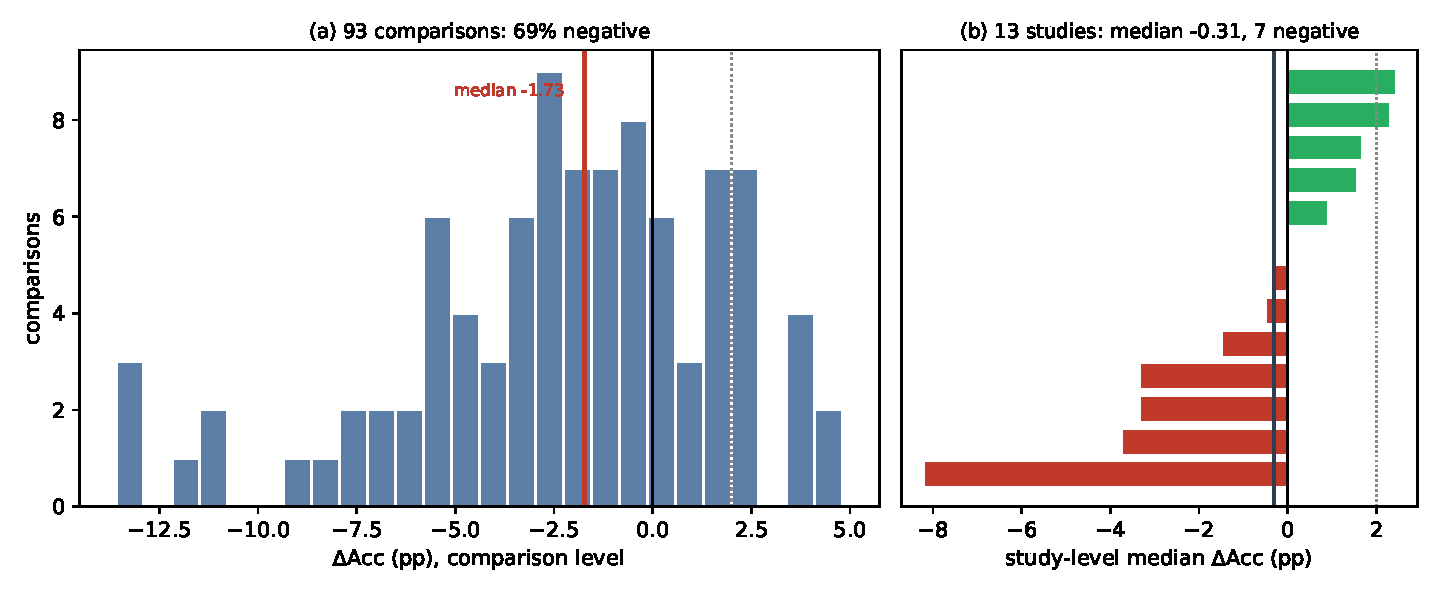
\includegraphics[width=0.84\textwidth]{figs/fig4_strongbaseline.pdf}
\caption{(a) Distribution of the 93 peer-reviewed comparisons against the strongest
single-agent configuration reported in the same study; red line = comparison-level median
($-1.73$ pp), dotted line = the 2 pp threshold. (b) The same evidence aggregated to its unit
of inference: one median per study. Seven of thirteen study medians are negative and the
median of medians is $-0.31$ pp.}
\label{fig:strong}
\end{figure}

\begin{figure}[ht]\centering
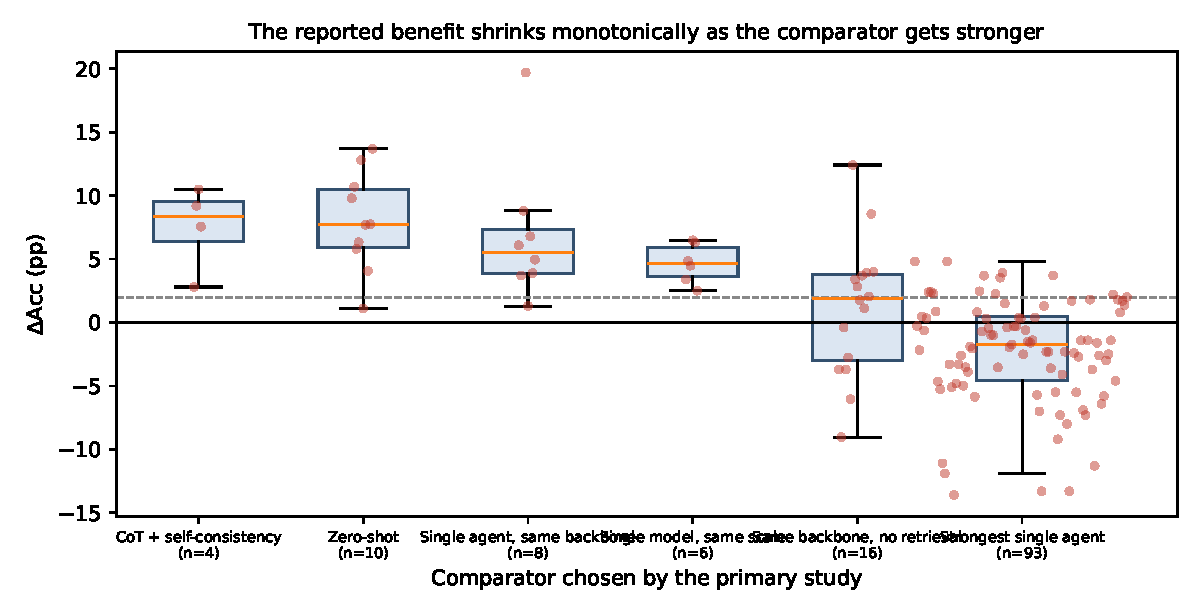
\includegraphics[width=\textwidth]{figs/fig1_comparator.pdf}
\caption{Each point is one extracted comparison; circles are peer-reviewed sources,
triangles preprints. The dashed line is the pre-specified interpretation threshold (2 pp).}
\label{fig:comparator}
\end{figure}


\paragraph{The largest controlled benchmark agrees.} MedAgentsBench \citep{tang2503}
evaluates four multi-agent methods and five single-agent prompting configurations across
nine medical datasets and four backbones, on a difficulty-curated hard subset (862 items).
Of its 108 comparisons against the strongest single-agent configuration in the same cell,
\textbf{78 (72\%) are negative}; restricted to the primary evaluation group
(MedQA, MedMCQA, the six MMLU medical subjects) the median is $-3.30$ pp with
\textbf{83\% negative}, and restricted further to the two discussion-based systems
(MedAgents, MDAgents) it is $-4.15$ pp with \textbf{92\% negative}.

\subsection{RQ2: more agents is not better, and a non-interactive control often wins}
The clearest within-paper evidence comes from \citet{yun2604} and \citet{mehrabi2606}, who
evaluate six single-agent experts, six-agent interactive baselines and their own systems on
the same MedMCQA slice (Table~\ref{tab:goa}).

\begin{table}[ht]\centering\small
\caption{MedMCQA accuracy under a common evaluation protocol and a common six-model pool
\citep{yun2604,mehrabi2606}. $\Delta$ is against the best single agent (55.22).}
\label{tab:goa}
\begin{tabular}{llrrr}
\toprule
System & Interaction & Agents & Acc. (\%) & $\Delta$ (pp) \\
\midrule
Best single agent (general)      & ---                & 1 & 55.22 & --- \\
Self-consistency                 & none (resampling)  & 1 & 55.70 & $+0.48$ \\
Self-MoA                         & homogeneous mixing & 6 & 55.56 & $+0.34$ \\
Mixture-of-Agents                & mixing             & 6 & 54.94 & $-0.28$ \\
Self-refine                      & iterative          & 6 & 54.94 & $-0.28$ \\
ReConcile                        & debate + confidence& 6 & 54.60 & $-0.62$ \\
Multi-agent debate               & debate             & 6 & 53.05 & $-2.17$ \\
Graph-of-Agents (selected)       & graph message pass & 3 & 60.04 & $+4.82$ \\
Relational aggregation           & structured passing & 6 & 62.83 & $+7.61$ \\
\bottomrule
\end{tabular}
\end{table}

Two observations follow. First, \emph{interaction per se does not pay}: four of the six
interactive six-agent baselines score below the best single agent, while non-interactive
self-consistency --- which requires no communication protocol at all --- is slightly
positive. Second, \emph{agent count is not the lever}: the best-performing configuration in
this pool uses three selected agents and outperforms six-agent systems, consistent with the
authors' own framing.

\paragraph{Orchestrating small models loses to simply using a bigger one.}
The sharpest statement of the balance problem comes from S-DAG \citep{wang2511}, which
evaluates six multi-model orchestration methods on MedMCQA using a pool of 7--13B experts,
alongside single-model chain-of-thought baselines at several scales. Measured against a
\emph{same-scale} single 7B model (72.07\%), every orchestration method is positive:
median $+4.67$ pp (range $+2.51$ to $+6.48$). Measured against the strongest single model
in the same table --- Qwen2.5-72B with plain chain-of-thought at 80.44\% --- \emph{every
one of them is negative}: median $-3.71$ pp (range $-5.86$ to $-1.89$), including the
paper's own system at $-2.06$ pp.

Table~\ref{tab:sdag} makes the practical implication explicit: four to six orchestrated
calls to 7B models cost more than one call to a 72B model and deliver less accuracy. Any
balance claim that omits the larger single model as a comparator is therefore not a balance
claim at all.

\begin{table}[ht]\centering\small
\caption{The same six methods on MedMCQA, measured against two different comparators
\citep{wang2511}. The sign of every conclusion flips.}
\label{tab:sdag}
\begin{tabular}{lrrr}
\toprule
Method (pool of 7--13B experts) & Acc.\ (\%) & vs 7B single & vs 72B single \\
\midrule
Self-Refine      & 74.58 & $+2.51$ & $-5.86$ \\
MoE router       & 75.45 & $+3.38$ & $-4.99$ \\
MAD (debate)     & 76.55 & $+4.48$ & $-3.89$ \\
GraphRouter      & 76.92 & $+4.85$ & $-3.52$ \\
S-DAG (proposed) & 78.38 & $+6.31$ & $-2.06$ \\
Symbolic-MoE     & 78.55 & $+6.48$ & $-1.89$ \\
\midrule
\textbf{Median}  &       & $\mathbf{+4.67}$ & $\mathbf{-3.71}$ \\
\bottomrule
\end{tabular}
\end{table}

Backbone scale otherwise behaved inconsistently. In \citet{tang2311} the same architecture gained
$+9.8$ pp on GPT-3.5 and $+10.7$ pp on GPT-4 over a zero-shot baseline, i.e.\ no attenuation
with scale, whereas \citet{su2509} show a 7B student with self-collaborative correction
reaching 71.3\% on CMExam, above its own 32B teacher (67.5\%). We therefore found no
consistent support for the hypothesis that smaller models benefit more; the evidence is
too sparse and too confounded by fine-tuning to decide.

\subsection{RQ3: what is bought, and at what price}
Figure~\ref{fig:pareto} plots $\Delta$Acc against the derived cost ratio. Cost could be
established for 110 of 293 comparisons, and in only 28 of those was it \emph{reported} by the
primary study rather than derived from the architecture description.
Typical multi-agent configurations sit at a median $R$ of $4\times$ (110 comparisons with a numeric cost ratio). The highest
cost-efficiency values are obtained by cheap mechanisms: \citet{tang2311} against a
self-consistency baseline ($\Delta=+9.2$ pp at $R\approx1.4$, $\mathrm{CEI}\approx19$) and
the two-stage self-correction of \citet{su2509} ($\Delta=+18.5$ pp at $R=2$,
$\mathrm{CEI}\approx18$). Large orchestrations buy proportionally less: at $R=20$ the
gain on hard items is $+9.0$ pp, i.e.\ $\mathrm{CEI}\approx2$.

\begin{figure}[ht]\centering
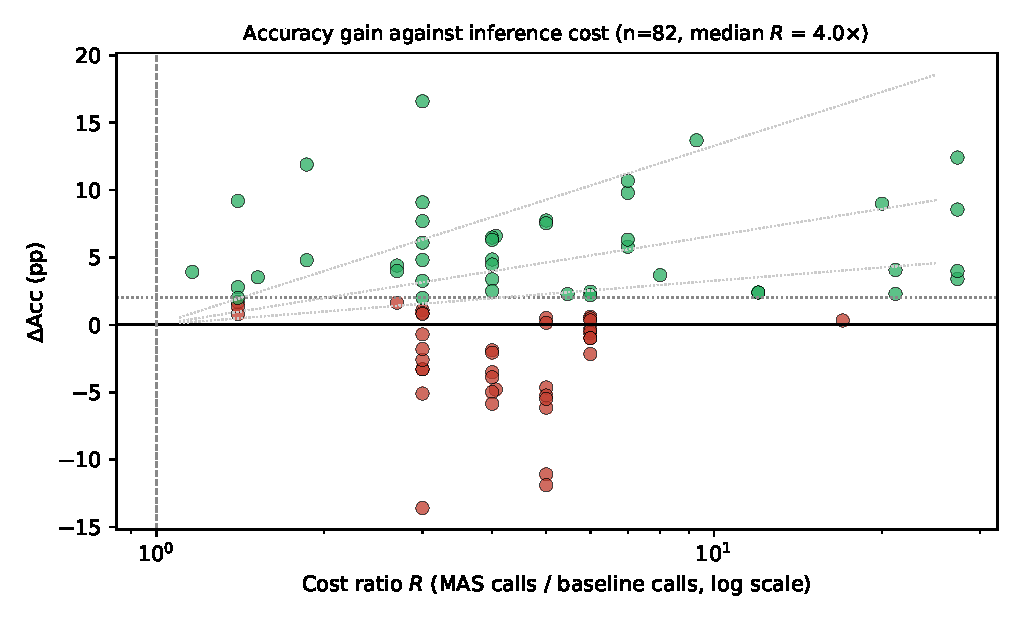
\includegraphics[width=0.86\textwidth]{figs/fig2_pareto.pdf}
\caption{Accuracy gain against derived cost ratio (log scale). Green points exceed the 2 pp
threshold, red points do not. Dotted lines are iso-efficiency contours.}
\label{fig:pareto}
\end{figure}

Two convergent data points concern aggregation. In \citet{chen2503} the multi-agent system
reaches 90.1\% on MedQA while \emph{Medprompt}, a single-agent prompting strategy, reaches
90.2\% on the same slice --- $-0.1$ pp for a substantially more complex system. In a
peer-reviewed licensing-examination study \citep{pm40336004}, an adaptive multi-agent
system reached 89.97\% while chain-of-thought plus few-shot prompting reached 87.67\%;
the authors themselves describe the latter as offering ``an optimal balance between
performance and efficiency'' because it achieves this ``with minimal API usage''. A
peer-reviewed agentic benchmark in \emph{npj Digital Medicine} \citep{pm41708802} reports
that adding agent enhancements moved accuracy from 24.0\% to 28.0\% on one clinical task
\emph{without statistical significance} --- a published null result of exactly the kind that
the preprint literature rarely contains.

\subsection{RQ4: gains concentrate on hard items}
\label{sec:rq4}
Two studies stratify gains by item difficulty, and they agree.

The medical evidence comes from MedLA \citep{ma2509}, which evaluates four published
multi-agent methods and a same-backbone LLaMA-3.1-8B single agent on the MedDDx benchmark
at three difficulty levels (Figure~\ref{fig:difficulty}). Excluding the proposing system,
the median gain is $\mathbf{-3.1}$ pp on \emph{Basic} items, $\mathbf{-2.2}$ pp on
\emph{Intermediate} items and $\mathbf{+1.4}$ pp on \emph{Expert} items. In other words,
on easy and moderate medical questions multi-agent collaboration is actively
\emph{harmful} relative to simply querying the same model once, and only at expert
difficulty does it turn positive --- and even then by less than the 2 pp threshold.
Majority voting is negative at all three levels.

The general-domain evidence agrees in direction and is larger in magnitude: scaling
test-time compute 15--20$\times$ buys $+2.2$ pp on easy items, $+8.5$ pp on medium items and
$+9.0$ pp on hard items \citep{wunderlich2605}; on easy items essentially nothing is bought
for a twentyfold cost.
The same study reports that mixture-of-agents reaches 71.4\% versus 64.3\% for
chain-of-thought, while self-consistency reaches 68.7\% and debate 70.0\% under comparable
compute --- again placing a non-interactive control within about one point of the
interactive methods.

\begin{figure}[ht]\centering
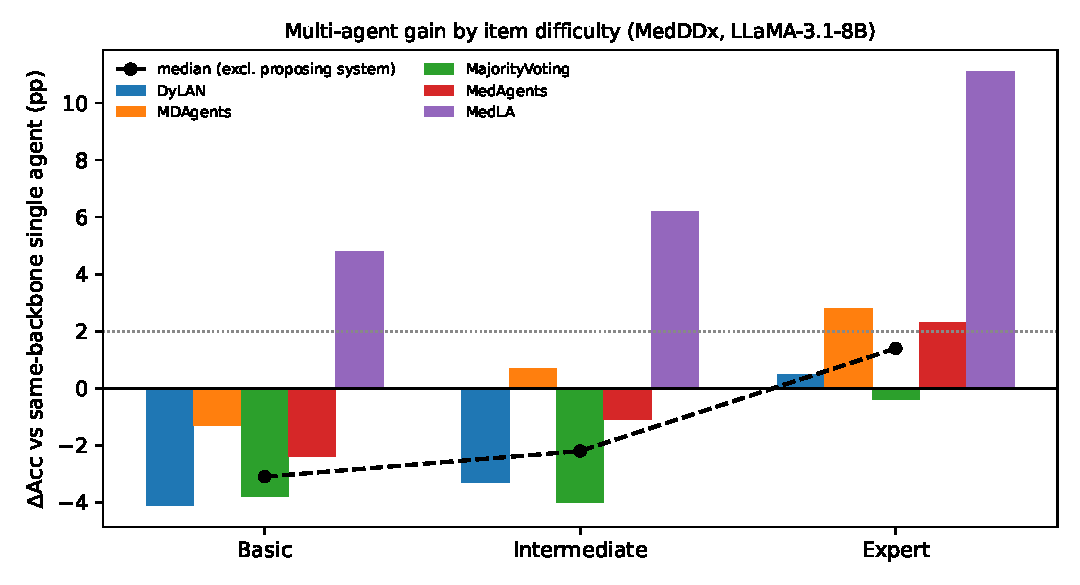
\includegraphics[width=0.78\textwidth]{figs/fig3_difficulty.pdf}
\caption{Multi-agent gain against a same-backbone single agent by item difficulty
(MedDDx, LLaMA-3.1-8B). The dashed line is the median across methods excluding the
proposing system: negative on Basic and Intermediate items, marginally positive on Expert
items. Data from \citet{ma2509}.}
\label{fig:difficulty}
\end{figure}

\subsection{Reporting practice}
Cost reporting remains the binding constraint: across 293 extracted comparisons a numeric
cost ratio exists for 110, and only 28 of those come from a figure the primary study
reported (API calls, tokens, USD or expert invocations); the remaining 82 were derived from
the architecture description, and 177 comparisons carry no usable cost information at all. Sampling
procedure --- whether the full test split or a subsample was used, and with what seed ---
was frequently unstated, which prevents several otherwise comparable results from being
placed in the same evaluation group.

\section{Discussion}

\subsection{Principal findings}
Three findings survive the analysis. (i) The headline accuracy gains reported for medical
multi-agent systems do not survive a fair comparator: measured against the strongest single
agent the same paper already ran, the study-level median is $-0.31$ pp with a 95\% CI of
$[-2.70, +0.36]$, i.e.\ no reproducible gain in either direction, and 69\% of individual
comparisons are negative. (ii) Non-interactive resampling
(self-consistency) is competitive with, and sometimes superior to, interactive debate and
mixing at comparable cost --- which means that a substantial part of the reported
``collaboration'' benefit is purchased compute rather than collaboration. (iii) What benefit exists is confined to hard items: on easy and moderate medical questions
the median effect against a same-backbone single agent is \emph{negative}
($-3.1$ and $-2.2$ pp), turning marginally positive ($+1.4$ pp) only at expert difficulty.

Taken together these support a simple practical rule: \emph{spend compute selectively on
hard items, prefer cheap aggregation, and always report what the strongest single agent
would have achieved}.

\subsection{Limitations of the evidence}
The included studies are now overwhelmingly peer-reviewed (280 of 293 extracted comparisons),
so the pattern cannot be attributed to preprint quality. It is instead attributable to
\emph{who chooses the comparator}: in almost every study the baseline is selected by the same
authors who propose the method, which is precisely the mechanism that produces finding (i).
The two studies that were explicitly designed as neutral benchmarks rather than as method
papers --- MedicalAgentsBench and MedAgentBoard --- are also the two that report the most
negative results. Cost is rarely measured. Variance is almost never
reported, so no pooled estimate with an interval is possible. Item-level results are
almost never released, which is why RQ4 rests on a single study and on a general-domain
benchmark rather than a medical one. Benchmark contamination is checked in a minority of
studies.

\subsection{Limitations of the review process}
\label{sec:limproc}
This draft deviates from its own protocol in ways that must be stated plainly.
The protocol was written but \textbf{not prospectively registered}. Screening, data
extraction and appraisal were performed by a \textbf{single reviewer} without duplicate
checking, and the formal risk-of-bias assessment specified in the protocol (six domains) has
\textbf{not} been completed.

\textbf{One study dominates.} MedicalAgentsBench contributes 36 of the 93 primary
comparisons; removing it moves the comparison-level median from $-1.73$ to $-0.60$ pp. The
sign is stable across all thirteen leave-one-study-out refits, the magnitude is not.

\textbf{Difficulty and benchmark are confounded.} A large share of the comparisons come from
deliberately hard-curated subsets on which every method operates near the floor, where paired
differences are noisier and systematically unlike full-test-split behaviour.

\textbf{Variances are essentially never recoverable}, so no pooled effect with a conventional
interval is possible; the bootstrap reported here propagates between-comparison and
between-study variation only, not within-comparison sampling error.

\textbf{The screened corpus came from two sources, not three.} 1{,}129 OpenAlex records were
retrieved but never entered the pre-specified triage rule because the API returns titles
without retrievable abstracts. A post hoc title-level screen of the 1{,}070 unscreened records
passed 0 on a three-facet screen and 3 on a two-facet screen, all clearly ineligible, so the
residual risk is small but the search sensitivity is bounded below rather than established.
The main search also required a supplementary round of probes to recover well-known systems
that the primary facet queries had missed.

\textbf{Retrieval remains incomplete.} Fifty subscription articles could not be retrieved,
and for a further 67 peer-reviewed articles only full text, not the publisher PDF, could be
obtained; both groups are recorded in the register for manual retrieval.

\textbf{Extraction is a convenience subset.} Of the studies for which a medical benchmark, a
baseline and extractable accuracies could all be identified, 30 contributed the 293 rows
analysed here; the remainder are registered and await extraction.

Accordingly this document should be read as a \textbf{preliminary synthesis} that fixes the
analytical frame and reports the signal visible in the extracted subset, not as a completed
systematic review.

Accordingly, this document should be read as a \textbf{preliminary synthesis} that fixes the
analytical frame and reports the signal visible in the first extracted subset, not as a
completed systematic review.

\subsection{Implications}
For method developers: report (a) the strongest single-agent baseline using the same
backbone, same evaluation items and same prompting budget; (b) an equal-budget
self-consistency control arm; (c) per-question calls, tokens and, where applicable, cost;
(d) item-level predictions. For reviewers and editors: a multi-agent result without a cost
figure and without a same-backbone strongest baseline is not interpretable.
For future reviews: the quantities that make synthesis possible --- paired item-level
outcomes and cost --- are precisely those that are missing, and that gap is itself the
most robust finding available today.

\section{Conclusion}
On the evidence retrievable today, the accuracy advantage of LLM multi-agent systems in
medical examination question answering is smaller than the literature suggests, is
concentrated on difficult items, and is frequently obtainable more cheaply by
non-interactive resampling. The field does not yet report enough cost information to
identify a balance point; making that reporting routine is the precondition for any
meaningful recommendation about which architecture to deploy.

\bibliographystyle{plainnat}
\bibliography{refs}

\appendix
\section{Data availability}
Search outputs (\texttt{search/}), triage and screening records (\texttt{screening/}),
the extracted comparison table (\texttt{extraction/data.csv}), analysis scripts
(\texttt{analysis/}) and the document register (\texttt{documents.md}) accompany this
draft.

\end{document}
